\chapter{Theory}
\section{The Operational Transconductance Amplifier}
The operational transconductance amplifier (OTA) is basically an op-amp without an output buffer. An OTA can be defined as an amplifier where all the nodes are low impedance except the input and output nodes. A schematic symbol of an OTA is shown in Figure.\ref{fig:OTA_symbol}. OTAs are generally programmable usually through the bias current that is provided to a differential amplifier. In the symbol, a bias voltage is being used as a programmable input. This bias voltage in turn controls the bias current of the amplifier. More on this later.

\begin{figure} [H]
\centering
\includegraphics[scale=1]{Figures/System_Level/OTA_Symbol.pdf}
\caption{Symbol of an OTA}
\label{fig:OTA_symbol}
\end{figure}

\subsection{Conventional Current Mirror OTA}
The schematic of a conventional current mirror based OTA is as shown in Figure.\ref{fig:OTA_Schematic_Ibias}. The OTA employs a differential input pair in conjunction with three current mirrors. The differential input pair comprises of transistors $M_1$ and $M_2$. The differential pair is biased by the current mirror formed by $M_{nB1}$ and $M_{nB2}$. PMOS current mirrors formed by $M_3$, $M_5$ and $M_4$, $M_6$ reflect currents generated in the differential pair on to the output shell. The current generated by the mirror formed by $M_3$ and $M_5$ is reflected to the output via the NMOS currentn mirror formed by $M_7$ and $M_8$. The current mirror gain factor is K. Increase in K will increase the slew rate and gain bandwidth along with the output current of the conventional OTA at the cost of increased area, static power dissipation and a decrease in phase margin.

\begin{figure} [H]
\centering
\includegraphics[scale=1]{Figures/Schematics/OTA_NMOS.pdf}
\caption{Schematic of a Conventional Current Mirror OTA}
\label{fig:OTA_Schematic_Ibias}
\end{figure}

Common mode signals are ideally rejected. i.e., when $V_{in+} = V_{in-}$, $I_{out}$ = 0. A differential input signal will generate an output current proportional to the applied differential voltage based on the transconductance of the differential pair. And that is why OTA is known as Voltage controlled Current Source. Although the output stage is push-pull structure, the conventional OTA is only capable for producing an output current with a maximum amplitude equal to the bias current in the output shell, provided the current mirror gain is unity, i.e., K=1. For this reason, conventional OTA is referred to as a Class A amplifier. 

The conventional OTA does not employ an output buffer and hence is only capable of driving capacitive loads and the capacitive load consumes all the current generated in the circuit. The gain of the OTA ($G_mR_o$) is dependent on the large output resistance of the output shell of the OTA formed by the transistors $M_3$ to $M_8$. The output resistance is reduced to $G_mR_o//R_L \approx G_mR_L$ if a parallel resistive load $R_L$ is applied.

Let us consider a hypothetical scenario that we do not need a resistive load to be driven as part of the system. In other words, we have a capacitive load as part of the specification. An advantage of this would be the fact that the need of an output buffer is eliminated and thereby the static power dissipation and the area occupied is reduced. But on the downside, the  amplifier behaviour for the output current would be like that of a band pass filter. So this scenario will not be useful as the specification demands a bandwidth of 10MHz as the overall system would be targetting low frequency applications. So a capacitive load will limit the output current only to a certain band of frequencies and hence it will not make sense to just use a one stage design. This gives rise to design an output buffer for the OTA.

An output buffer can either be a voltage buffer or a current buffer depending on how the OTA is designed. A current buffer, for example, is used to hold the output current of the OTA at the output of the buffer. So any amplification needed for this current would in turn give rise to the need of another stage, making the design complicated. In this case usually a current feedback amplifiers are designed which theoretically has a low input impedance non-inverting terminal input and a high input impedance inverting terminal input. So the OTA output would directly be connected to this non-inverting terminal and with the use of internal buffers, the output current follows the input current.

In this work, however, a voltage buffer amplifier is designed. Therefore, the OTA is used as a programmable block to control the output voltage rather than the output current.

\subsection{Other Topologies}
The Conventional OTA considered in the previous section is a Class A type of amplifier. These amplifiers can produce output currents that are equal to the bias currents for a unity current mirror gain. Need for high speed and high current with low power dissipation gave rise to research in Class AB Amplifiers. There are many topologies of the Class AB type OTAs that are classified based on their structure as:
\begin{itemize}
\item Folded Cascode OTA
\item Telescopic OTA
\item Local Common Mode Feedback OTA
\item Cascode Voltage Flipped Follower based OTA
\end{itemize}

One of the figures of merit to compare these OTAs is the Current Enhancement factor (CE). $CE = I_{out-max}/2I_{bias}$. Class A amplifiers typically have a CE of 1. Class AB OTAs have a high CE value. A family of OTA denoted as $Super Class-AB OTA$ have remarkably large CE values. Typical value of CE ranges from 100 to 500 depending on the implementation of the Class-AB differential pair and the output branches. Cascode Voltage Flipped Follower based OTA is one such example of a Super Class-AB OTA. These OTAs have the largest reported CE in literature. Some of the OTA designs considered are explained in the next chapter.

\vfill
\clearpage

\section{The Opeartional Amplifier}
The operational amplifier (OP AMP) is a fundamental building block in analog integrated circuit design. A typical symbol of an OP AMP is as shown in Figure.\ref{fig:OPAMP_symbol}. It consists of differential input terminals - inverting ($V_{in-}$) and non-inverting ($V_{in+}$), a positive supply pin ($V_{DD}$) and a negative/ground supply pin ($V_{SS}$) and the output terminal ($V_{out}$). Simple OP AMPs are generally used as Summing amplifier, differentiator, integrator, transimpedance amplfier, and so on. OP AMPs with vastly different levels of complexity are used to realize functions ranging from dc bias generation to high-speed amplification or filtering.

\begin{figure} [H]
\centering
\includegraphics[scale=1]{Figures/System_Level/OPAMP_Symbol.pdf}
\caption{Symbol of an OP AMP}
\label{fig:OPAMP_symbol}
\end{figure}

OP AMPs are voltage controlled voltage sources, much to the contrary of OTAs, which are voltage controlled current sources. Design of an OP AMP consists of determining the specifications, selecting the device sizes and biasing conditions, compensating the op-amp for stability, simulating and characterizing the open loop gain, the input common mode range, common mode rejection ratio, power supply rejection ration, output votlage range, current sourcing/sinking capability and power dissipation.
OP AMPs are used as a voltage buffer whenever there is a need to drive resistive loads or a combination of capacitive load and a resistive load.

\subsection{Miller Compensation OP AMP}
The schematic of the a two-stage Miller Compensation OP AMP is as shown in Figure.\ref{fig:OPAMP_Schematic_Ibias}. First stage of the OP AMP is the differential amplfier formed by the transistors $M_1-M_5$ and $M_8$. The second stage of the OP AMP is the Common Source amplifier formed by the transistors $M_6$ and $M_7$. Compensation Capacitor or Miller Capacitor denoted by $C_C$ is used for the splitting of the poles of the two stages thereby providing stability and also controlling the bandwidth and the slew rate. 
\begin{figure} [H]
\centering
\includegraphics[scale=1]{Figures/Schematics/OPAMP_Ibias.pdf}
\caption{Schematic of a Two-stage Miller Compensation OP AMP}
\label{fig:OPAMP_Schematic_Ibias}
\end{figure}
The biasing to the differential input pair is provided by the current mirror formed by $M_5$ and $M_8$. The selection of the bias current, $I_{bias}$ is determined by gain, ICMR, CMRR, power dissipation, noise, slew rate and matching considerations. If slew-rate is of concern, a cross-coupled differential amplifier should be considered for the first stage. The second stage common source amplifier is used to provide an additional gain to the overall OP AMP since the gain provided by the differential pair is usually not large enough. It is known that OP AMPs have infinitely large open loop gain. This second stage also provided a current boosting since $M_7$ forms a current mirror with $M_8$ and the dimensions of $M_7$ are usually larger than $M_8$, thereby setting the current at the output of the OP AMP. The best use of these OP AMPs are made as part of voltage buffers. i.e., the OP AMP is connected in unity gain configuration by providing a direct feedback from the output terminal to the non-inverting terminal.
\vfill
\clearpage
\section{The Gm/Id Methodology}

Good analog design is an art, not a science. Best work are still done on napkins and not on EDA tools, i.e., using Hand Calculations. However in recent times, in most cases at least, the equations which were once valid have become inadequate. The ability of these equations are limited to only certain cases. The famous equation for $I_{ds}$ is naturally the first thing that comes to mind when someone says Square Law, which is given by 
$$I_{ds} = \frac{\mu \cdot C_{ox}\cdot W}{2\cdot L}.(V_{gs}-V_{th})^2$$

The square law becomes linear in short-channel limit and thus they are suitable only for long channel MOSFETs. The block diagram in Figure.\ref{fig:Square_Law} indicates the failure in Square law, especially in deep submicron technologies.

\begin{figure} [H]
\centering
\includegraphics[scale=1]{Figures/Misc/PDFs/Square_Law.pdf}
\caption{Square Law Methodology}
\label{fig:Square_Law}
\end{figure}

The values obtained from hand calculations for short channel MOSFETs are far away from accuracy according to the requirements and thus there will be a huge gap in the spice simulation results and the specifications. The reason why this methodology has still not been a disaster is that fact that it over-predicts the $V_{dsat}$, but keeps the transistors in saturation. But in strong saturation, the gain from the MOSFET is not very high. So this methodology skips the possibility of fine-tuning the device in the nascent stages of design.

The $G_m$/$I_D$ methodology on the other hand, is fundamentally more practical than theoretical. This methodology uses pre-computed spice data in hand calculation, thereby providing accurate results. The diagram in Figure.\ref{fig:GmID} shows that this methodology uses design tables which are pre-computed and using those tables, the hand calculations are made, which are rather simple and straight forward. 

\begin{figure} [H]
\centering
\includegraphics[scale=1]{Figures/Misc/PDFs/GmID.pdf}
\caption{Gm/ID Methodology}
\label{fig:GmID}
\end{figure}

To obtain the design tables, we need to look at a transistor in terms of width-independent figures of merit that are linked to the design specification. The design trade-offs have to be considered in terms of MOSFET's inversion level by using $G_m$/$I_D$ as a proxy. The circuit in Figure.\ref{fig:GmID_Ckt} is used to simulate the figures of merit parameters that are necessary to make design decisions. The width of the transistor $M_0$ is set to 5$\mu$m and the length is kept as a variable. The value of $V_{ds}$ is set to a value that is half of the value of the power supply. As part of this work, the supply we use is +2.5V and -2.5V. So technically we have a voltage difference of 5V and therefore, the value of $V_{ds}$ is set to 2.5V.

\begin{figure} [H]
\centering
\includegraphics[scale=1]{Figures/Misc/PDFs/GmID_NMOS.pdf}
\caption{Setup for simulating GmID parameters}
\label{fig:GmID_Ckt}
\end{figure}
The ocean script used to simulate this circuit and to obtain the data which is used to generates the graphs below is attached in the Appendix A. The figures of merit considered as part of this work for $G_m$/$I_D$ methodology are $G_m$/$I_D$, $f_T$(transit frequency), $G_m$/$G_{ds}$(intrinsic gain), $I_D$(drain current), $f_TG_m$/$I_D$ (design trade-off).

\begin{figure} [H]
\centering
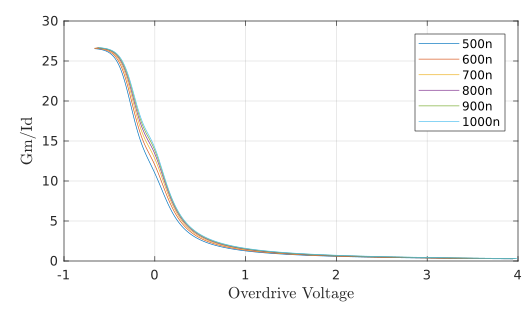
\includegraphics[scale=1]{Figures/Misc/PDFs/nmos_len_vovgmid.pdf}
\caption{$G_m$/$I_D$ vs $V_{ov}$}
\label{fig:vovgmid}
\end{figure}

The plot of $G_m$/$I_D$ versus the Overdrive voltage is shown in Figure.\ref{fig:vovgmid}. 
The value of $G_m$/$I_D$ is very high when the overdrive voltage is less than zero, i.e., when the transistor is in weak inversion. The gain starts dropping with increase in overdrive voltage and it becomes close to zero and constant and theat is where the transistor goes into strong inversion. The response to variation in length is minimal for this parameter.

\begin{figure} [H]
\centering
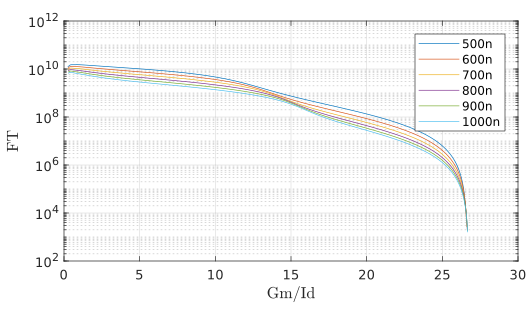
\includegraphics[scale=1]{Figures/Misc/PDFs/nmos_len_gmidft.pdf}
\caption{$f_T$ vs $G_m$/$I_D$}
\label{fig:gmidft}
\end{figure}

Transit frequency is defined as the ratio of the transconductance $G_m$ to its gate to source capacitance $C_{gs}$. The plot of transit frequency against $G_m$/$I_D$ is as shown in Figure.\ref{fig:gmidft}. The figure of merit is used to indicate the speed of operation of the MOSFET. And from the plot, it can be seen that the speed is high when the value of $G_m$/$I_D$ is low. So this is quite the opposite to the gain parameter that was discussed with the previous plot. So here we have our first trade-off between high gain and high speed.

\begin{figure} [H]
\centering
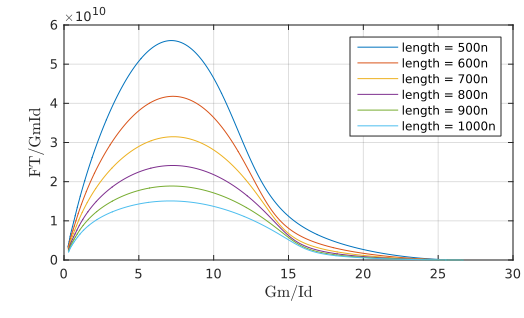
\includegraphics[scale=1]{Figures/Misc/PDFs/nmos_len_gmidftgmid.pdf}
\caption{$f_TG_m/I_D$ vs $G_m$/$I_D$}
\label{fig:gmidftgmid}
\end{figure}

To evaluate the trade-off mentioned above, the product of the two figures of merit are considered and then plotted against the $G_m$/$I_D$ parameter and is plotted as shown in Figure.\ref{fig:gmidftgmid}. The product is highest in moderate inversion. And this is called as the sweet spot and this provides the best possible trade-off between gain and speed. This is something that cannot be obtained using the square law as moderate inversion range is never utilized in that methodology.

\begin{figure} [H]
\centering
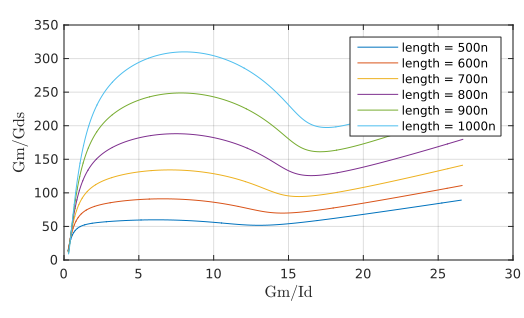
\includegraphics[scale=1]{Figures/Misc/PDFs/nmos_len_gmidgmgds.pdf}
\caption{$G_m/G_{ds}$ vs $G_m$/$I_D$}
\label{fig:gmidgmgds}
\end{figure}

The intrinsic gain $G_m/G_{ds}$ is plotted against $G_m$/$I_D$ as shown in Figure.\ref{fig:gmidgmgds}. This along with Figure.\ref{fig:gmidft} form a powerful tool in choosing the value of the channel length that meets the gain requirements. The plot in Figure.\ref{fig:vovgmid} did not show too much of a variation with respect to length. But using this plot it is easy to decide the channel length of the transistor. It is clear that the smallest channel length in moderate inversion provide the highest gain with a decent trade-off with respect to speed, i.e., transist frequency.

\begin{figure} [H]
\centering
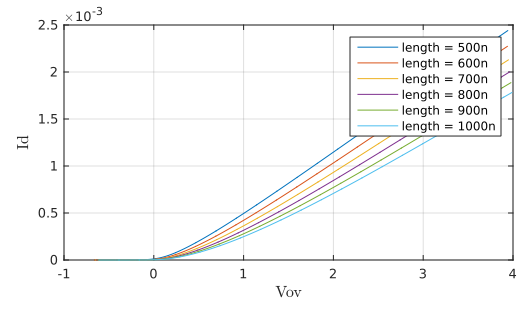
\includegraphics[scale=1]{Figures/Misc/PDFs/nmos_len_vovid.pdf}
\caption{$I_D$ vs $V_{ov}$}
\label{fig:vovid}
\end{figure}

The final plot we have here is to choose the drain current for the overdrive voltage needed. It is as shown in Figure.\ref{fig:vovid}. Ultimately, it is the overdrive voltage that determines the region of operation of the transistor. So with the overdrive voltage known and the length of the transistor decided, the drain current can be easily chosen.

An important thing not to forget is that the figures of merit simulated and plotted are independent of variation in the width of the transistor. So once, the other parameters are decided, the value of W can be chose using the Id/W plot. The steps involved in the general design flow of this methodology is summarized below.
\begin{itemize}
\item Determine $G_m$ from (design objectives)
\item Pick the channel length L
	\begin{itemize}
	\item Short channel $\rightarrow$ high $f_T$ (high speed)
	\item Long channel $\rightarrow$ high intrinsic gain
	\end{itemize}
\item Pick $G_m$/$I_D$ (or $f_T$)
	\begin{itemize}
	\item Large $G_m$/$I_D$ $\rightarrow$ low power, large signal swing
	\item Small $G_m$/$I_D$ $\rightarrow$ high $f_T$ (high speed)
	\end{itemize}
\item Determine $I_D$ (from $G_m$ and $G_m$/$I_D$)
\item Determine W (from $I_D$/W)
\end{itemize}

There are many other possibilities to design using this methodology and this depends the specifications, constraints and objectives. However, as part of this thesis the steps mentioned above are followed and the plots discussed above are used to design the differential pair of transistors for all the stages of the system. And the other transistors' dimensions were finalized using simulation and output results.